% Breadboard wiring diagrams for the control system build, drawn one step at a
% time. Each wiring-step-N.tex is a standalone wrapper that calls
% \wiringdiagram{N}: parts from earlier steps are drawn faded, the parts added
% in step N are drawn in full, and later steps are left out. wiring-complete.tex
% calls \wiringdiagram{0}, which draws the finished board with nothing faded.
%
% Steps: 1 power + ready LED (D4), 2 crank sensor (D2) + crank LED (D5),
% 3 wheel sensor (D3) + wheel LED (D7), 4 motor LED (D6) + servo (D9),
% 5 motor driver (D10).
%
% Coordinates are in breadboard hole pitches, with the board drawn landscape
% (rotated 90 degrees, as in the lab 2-4 slides), so row 1 is on the left and
% column j is at the top. The hole positions were measured off breadboard.png:
% row r sits at x = 1.356 + r, and the columns and rails sit at the heights
% below. The power rail holes come in groups of five: under rows 1-5, 7-11,
% 13-17, 19.6-23.6 (this group is offset by just over half a hole) and 26-30.
%
% The Nano covers rows 1-15, pins in columns g (top) and c (bottom):
%   top    row: 1 D12, 2 D11, 3 D10, 4 D9, 5 D8, 6 D7, 7 D6, 8 D5, 9 D4,
%               10 D3, 11 D2, 12 GND, 13 RST, 14 RX0, 15 TX1
%   bottom row: 1 D13, 2 3V3, 3 AREF, 4-11 A0-A7, 12 +5V, 13 RST, 14 GND, 15 VIN
%
% Things that plug in from off the board (sensors, servo, motor driver) are
% drawn above it, with their wires passing between the rail holes.

\usetikzlibrary{calc}

\newlength{\pitch}
\setlength{\pitch}{0.42cm}
\expandafter\def\csname col-a\endcsname{4.745}
\expandafter\def\csname col-b\endcsname{5.746}
\expandafter\def\csname col-c\endcsname{6.746}
\expandafter\def\csname col-d\endcsname{7.745}
\expandafter\def\csname col-e\endcsname{8.747}
\expandafter\def\csname col-f\endcsname{11.745}
\expandafter\def\csname col-g\endcsname{12.747}
\expandafter\def\csname col-h\endcsname{13.746}
\expandafter\def\csname col-i\endcsname{14.746}
\expandafter\def\csname col-j\endcsname{15.747}
% power rails: top + is the inner one, top - the outer; the bottom pair is
% the other way round
\expandafter\def\csname col-tp\endcsname{17.947}
\expandafter\def\csname col-tm\endcsname{19.147}
\expandafter\def\csname col-bm\endcsname{2.946}
\expandafter\def\csname col-bp\endcsname{1.746}

% \hole{row}{column}: the centre of a hole, e.g. \hole{9}{h} or \hole{14}{bm}
\newcommand{\hole}[2]{({1.356+(#1)},{\csname col-#2\endcsname})}
% \col{column}: just the height of a column
\newcommand{\col}[1]{\csname col-#1\endcsname}
% \rowx{row}: just the x position of a row
\newcommand{\rowx}[1]{{1.356+(#1)}}

% wire colours: red for +5V, black for GND, yellow for signals. The servo
% keeps its own cable colours (brown, red, orange), as in lab 3, and the motor
% driver's AIN1 wire is blue, as on the rig's cable
\definecolor{signal}{RGB}{245,195,0}
\definecolor{ain1}{RGB}{30,110,230}
\definecolor{pcb}{RGB}{28,58,135}

\tikzset{
    jumper/.style={line width=.9mm, rounded corners=.9mm},
    jumper5v/.style={jumper, draw=Red},
    jumpergnd/.style={jumper, draw=black},
    leg/.style={line width=.6mm, draw=DimGray},
    lead/.style={line width=.7mm, rounded corners=.9mm},
    lead5v/.style={lead, draw=Red},
    leadgnd/.style={lead, draw=black},
    leadsig/.style={lead, draw=signal},
    label/.style={font=\sffamily\footnotesize, text=black, inner sep=1pt},
    pinlabel/.style={font=\sffamily\tiny, text=white, inner sep=0pt},
    nanolabel/.style={font=\sffamily\bfseries\fontsize{4}{4}\selectfont,
        text=black, fill=white, rounded corners=.3mm, inner sep=.5pt},
}

% a tag naming a Nano pin, on the board just inside the pin
\newcommand{\toppin}[2]{% #1 row, #2 pin name
    \node[nanolabel] at (\rowx{#1}, {\col{g}-0.85}) {#2};
}
\newcommand{\bottompin}[2]{% #1 row, #2 pin name
    \node[nanolabel] at (\rowx{#1}, {\col{c}+0.85}) {#2};
}

% a resistor lying along a column, between two rows
\newcommand{\resistor}[4]{% #1 image, #2 column, #3 first row, #4 last row
    \draw[leg] \hole{#3}{#2} -- \hole{#4}{#2};
    \node[inner sep=0] at ({1.356+((#3)+(#4))/2}, \col{#2})
        {\includegraphics[width=1.9\pitch]{#1}};
}
% a resistor across the centre channel, from column f to column e of one row
\newcommand{\channelresistor}[2]{% #1 image, #2 row
    \draw[leg] \hole{#2}{f} -- \hole{#2}{e};
    \node[inner sep=0, rotate=90] at (\rowx{#2}, {(\col{e}+\col{f})/2})
        {\includegraphics[width=1.9\pitch]{#1}};
}
% a resistor from column j of one row straight up into the top + rail
\newcommand{\railresistor}[2]{% #1 image, #2 row
    \draw[leg] \hole{#2}{j} -- \hole{#2}{tp};
    \node[inner sep=0, rotate=90] at (\rowx{#2}, {(\col{j}+\col{tp})/2})
        {\includegraphics[width=1.6\pitch]{#1}};
}
% a patch cable lying loose over the board between two holes, drawn as a
% gentle curve in the same style as the leads, with a thin white edge that
% only shows where it passes over another wire
\newcommand{\patch}[5][10]{% #1 bend angle, #2 #3 from row and column,
                            % #4 #5 to row and column
    \draw[line width=1.2mm, draw=white, line cap=round, shorten <=.4mm,
        shorten >=.4mm]
        (\rowx{#2}, \col{#3}) to[bend left=#1] (\rowx{#4}, \col{#5});
    \draw[line width=.7mm, draw=signal, line cap=round]
        (\rowx{#2}, \col{#3}) to[bend left=#1] (\rowx{#4}, \col{#5});
}
% an LED standing between a hole in column a and a hole on the bottom - rail,
% with a label under the board
% (the body sits square under its row, so a row of LEDs lines up evenly
% whatever rail holes their legs reach for)
\newcommand{\led}[3]{% #1 row in column a, #2 position along the rail, #3 label
    \draw[leg] \hole{#1}{a} -- (\rowx{#1}, 3.846) -- \hole{#2}{bm};
    \draw[draw=gray, line width=.2mm] (\rowx{#1}, 3.2) -- (\rowx{#1}, -0.3);
    \filldraw[fill=red, draw=black, line width=.3mm]
        (\rowx{#1}, 3.846) circle (.55);
    \node[label, anchor=north, font=\sffamily\scriptsize]
        at (\rowx{#1}, -0.3) {#3};
}
% a wire from something off the board: down from its pin at x=#2, across to
% x=#3 (between the rail holes), down to height #4, then into hole #5
\newcommand{\offboard}[5]{%
    \draw[#1] (#2, 23.2) -- (#2, 22.6) -- (#3, 21.6) -- (#3, #4) -- #5;
}
% a Hall effect sensor on a lead, centred at x=#1, pins 0.5 apart
\newcommand{\sensor}[2]{% #1 centre, #2 label
    \filldraw[fill=black] ({#1-1.1}, 23.2) -- ({#1+1.1}, 23.2)
        -- ({#1+0.8}, 24.6) -- ({#1-0.8}, 24.6) -- cycle;
    \node[pinlabel, font=\sffamily\scriptsize] at (#1, 23.9) {A3144};
    \node[label, anchor=south] at (#1, 24.7) {#2};
}

% draws #2 as part of step #1: faded before the current step, in full on it,
% and not at all after it. Step 0 is the completed board, with everything
% drawn in full
\newcommand{\forstep}[2]{%
    \ifnum\wiringstep=0
        #2%
    \else\ifnum#1<\wiringstep
        \begin{scope}[transparency group, opacity=.3]#2\end{scope}%
    \else\ifnum#1=\wiringstep
        #2%
    \fi\fi\fi
}

\newcommand{\wiringdiagram}[1]{%
\def\wiringstep{#1}%
\begin{tikzpicture}[x=\pitch, y=\pitch]
    %% breadboard and Nano: rows 1-15, USB end hanging off the left
    \node[anchor=south west, inner sep=0] at (0, 0)
        {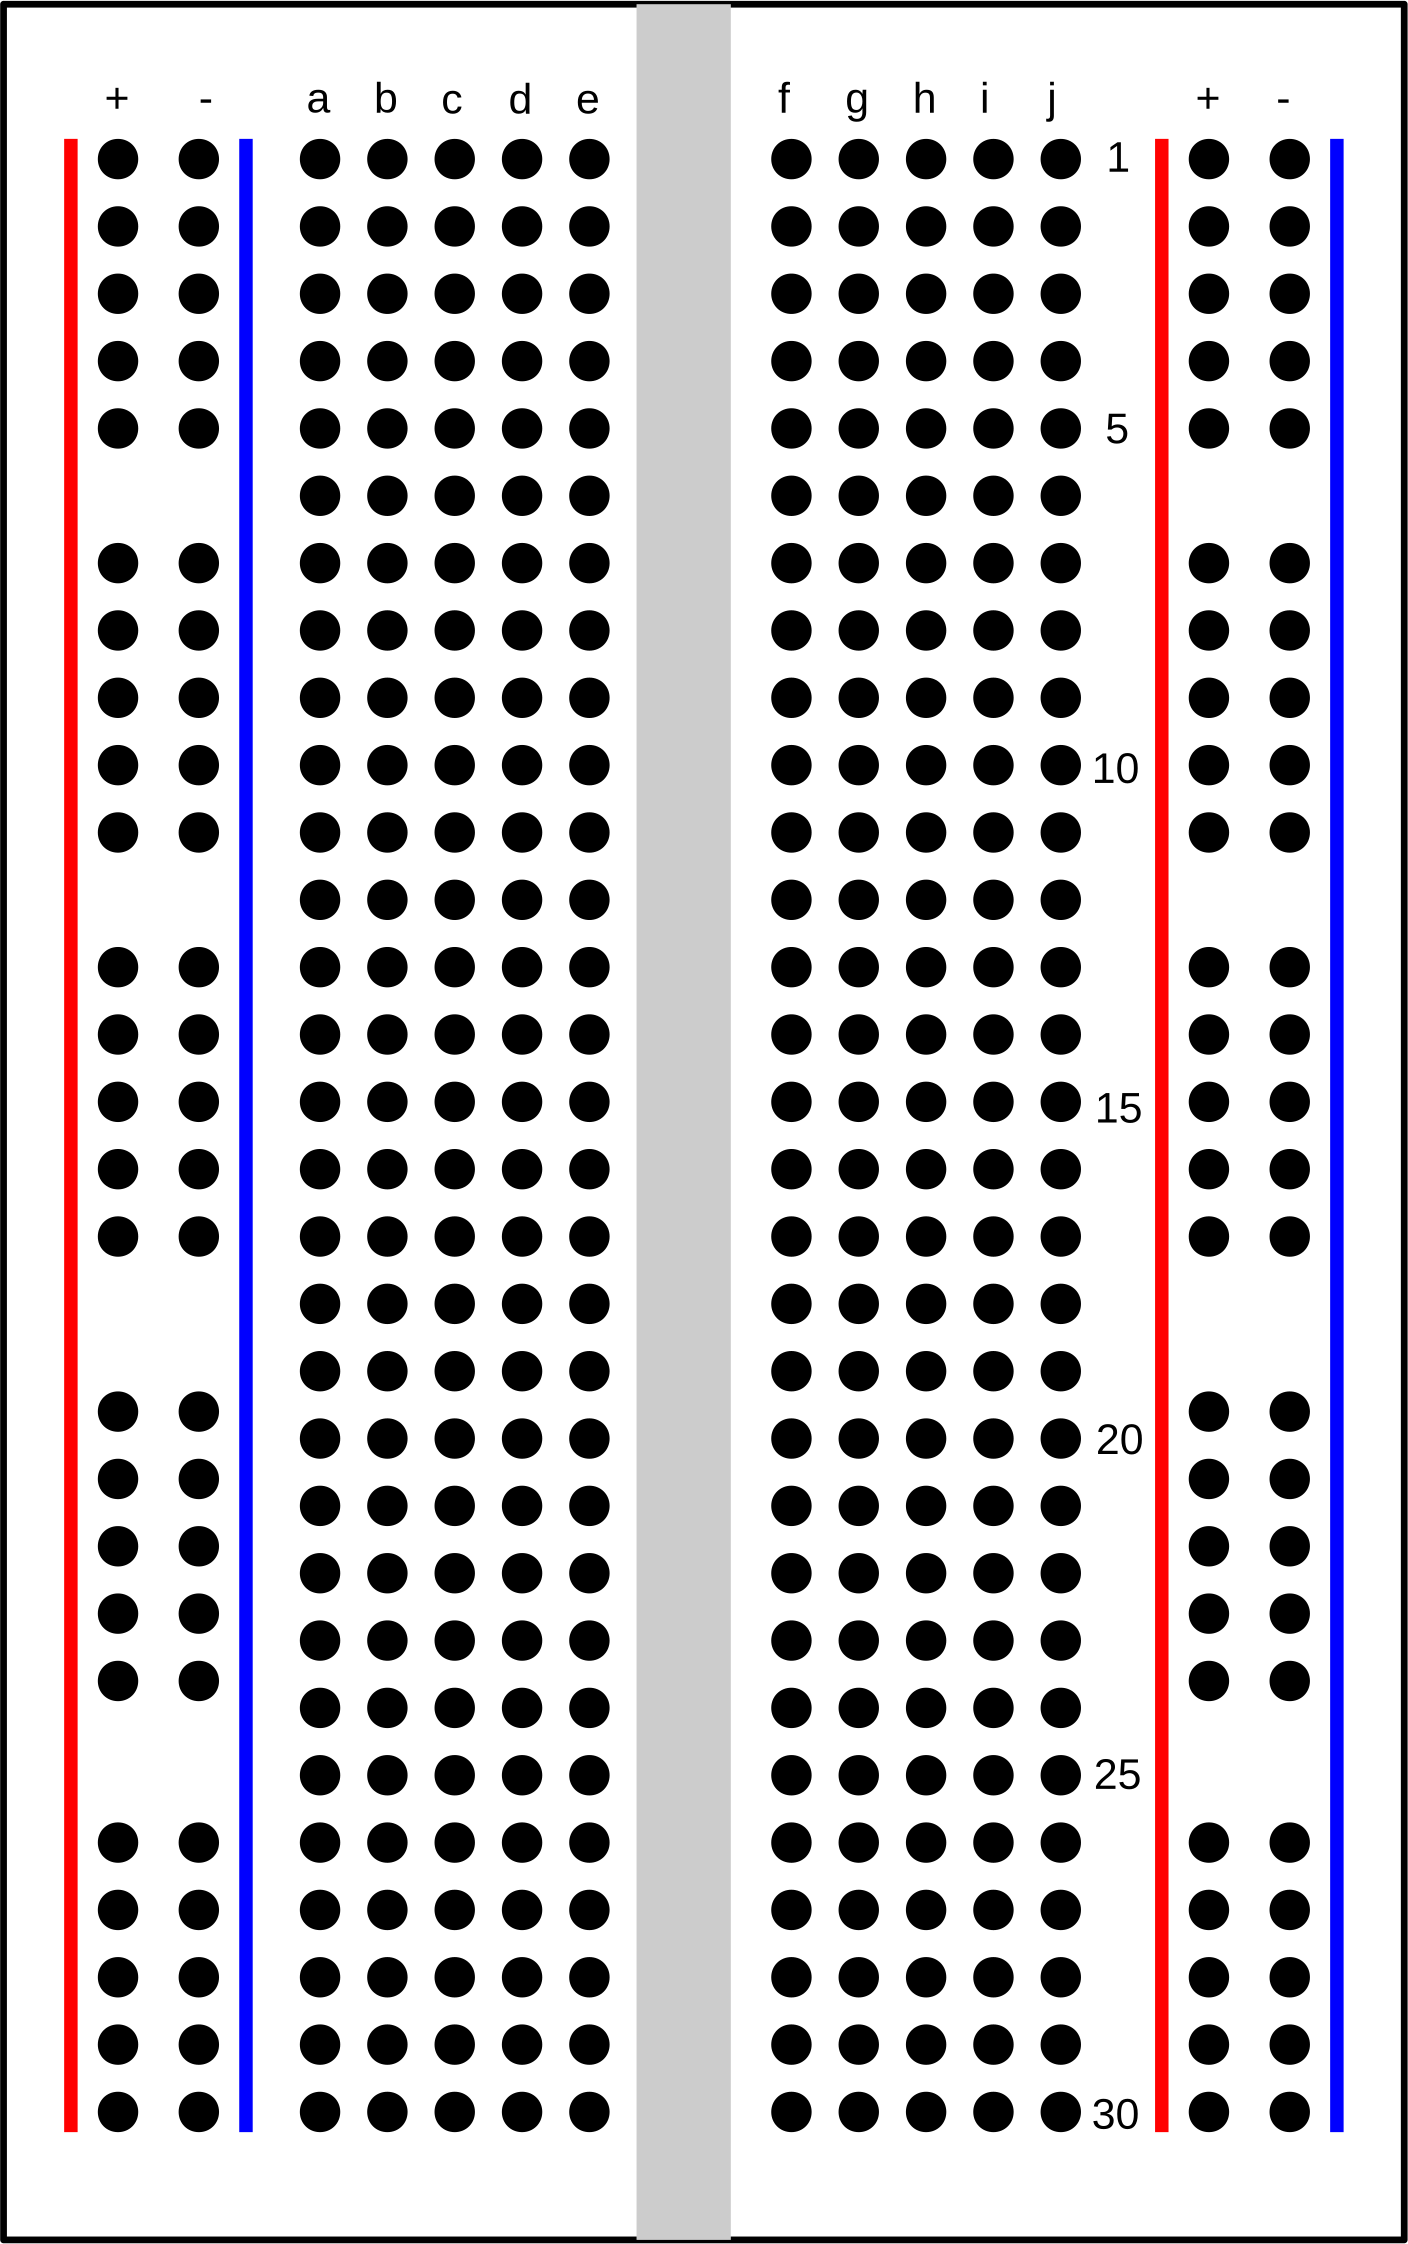
\includegraphics[angle=90, width=33.32\pitch]{breadboard.png}};
    \node[anchor=north west, inner sep=0] at (-0.276, 13.274)
        {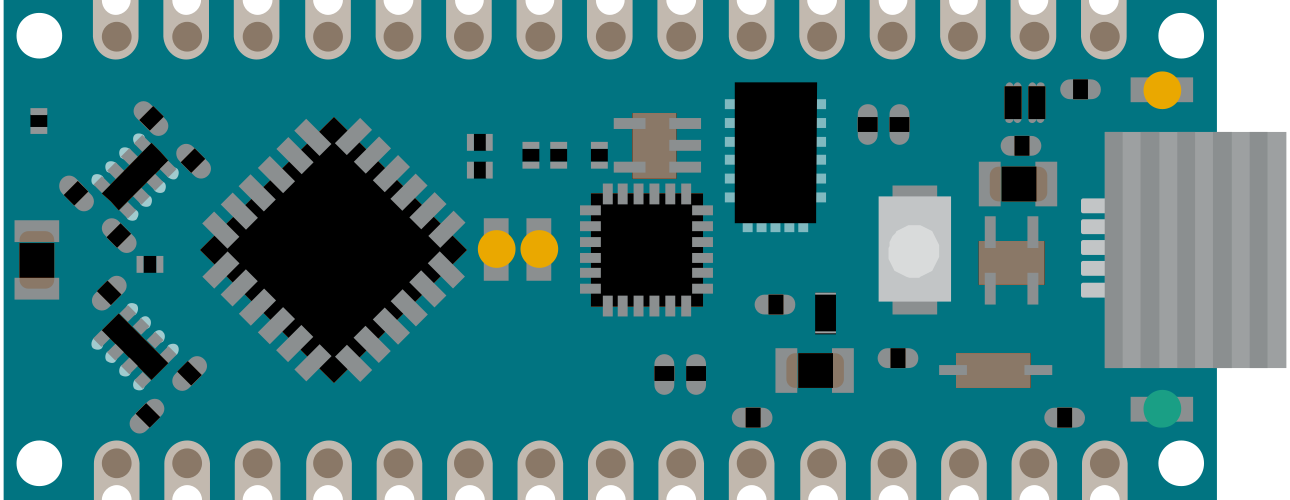
\includegraphics[angle=180, width=18.284\pitch]{nano.png}};

    %% step 1: power rails and the system ready LED (D4)
    \forstep{1}{
        % GND and +5V from the Nano to the bottom rails
        \draw[jumpergnd] \hole{14}{a} -- \hole{14}{bm};
        \draw[jumper5v] \hole{12}{b} -- (\rowx{12}, 2.35) -- \hole{13}{bp};
        % carry both rails round to the top of the board
        \draw[jumper5v] \hole{30}{bp} -- (\rowx{29.5}, 2.35)
            -- (\rowx{29.5}, 17.35) -- \hole{30}{tp};
        \draw[jumpergnd] \hole{30}{bm} -- (\rowx{30.85}, \col{bm})
            -- (\rowx{30.85}, 18.55) -- (\rowx{30}, 18.55) -- \hole{30}{tm};
        % D4 -> 220 across the channel -> LED -> GND, all in row 18. The four
        % LEDs' GND legs share one group of rail holes (19.6-22.6)
        \patch[12]{9}{h}{18}{h}
        \channelresistor{resistor-220.png}{18}
        \led{18}{19.6}{ready}
        \bottompin{12}{5V}
        \bottompin{14}{GND}
        \toppin{9}{D4}
    }

    %% step 2: crank sensor on D2, and the crank activity LED (D5)
    \forstep{2}{
        % crank sensor straight into D2's own row (11): OUT in column i, and
        % the 10k pull-up from column j into the + rail. The sensor faces
        % away, so its OUT leg is on the left; GND is always the middle leg
        \railresistor{resistor-10k.png}{11}
        \sensor{15.356}{crank sensor}
        \offboard{leadsig}{14.856}{\rowx{11.5}}{15.0}{\hole{11}{i}}
        \offboard{leadgnd}{15.356}{\rowx{14}}{19.5}{\hole{14}{tm}}
        \offboard{lead5v}{15.856}{\rowx{14.5}}{18.55}{\hole{15}{tp}}
        % D5 -> 220 across the channel -> LED -> GND, all in row 20
        \patch[18]{8}{h}{20}{h}
        \channelresistor{resistor-220.png}{20}
        \led{20}{20.6}{crank}
        \toppin{11}{D2}
        \toppin{8}{D5}
    }

    %% step 3: wheel sensor on D3, and the wheel activity LED (D7)
    \forstep{3}{
        % wheel sensor straight into D3's own row (10), as for the crank
        % sensor; legs, left to right: +5V, GND, OUT
        \railresistor{resistor-10k.png}{10}
        \sensor{10.856}{wheel sensor}
        \offboard{lead5v}{10.356}{\rowx{8.5}}{18.55}{\hole{8}{tp}}
        \offboard{leadgnd}{10.856}{\rowx{9}}{19.5}{\hole{9}{tm}}
        \offboard{leadsig}{11.356}{\rowx{9.5}}{15.0}{\hole{10}{i}}
        % D7 -> 220 across the channel -> LED -> GND, all in row 22
        \patch[23]{6}{h}{22}{h}
        \channelresistor{resistor-220.png}{22}
        \led{22}{21.6}{wheel}
        \toppin{10}{D3}
        \toppin{6}{D7}
    }

    %% step 4: motor activity LED (D6) and the speedometer servo on D9
    \forstep{4}{
        % D6 -> 220 across the channel -> LED -> GND, all in row 24
        \patch[28]{7}{h}{24}{h}
        \channelresistor{resistor-220.png}{24}
        \led{24}{22.6}{motor}
        % servo on D9
        \filldraw[fill=blue, draw=black, line width=.3mm]
            (4.9, 23.2) rectangle (8.3, 24.8);
        \filldraw[fill=white, draw=black, line width=.3mm] (7.4, 24) circle (.55);
        \node[label, anchor=south] at (6.6, 24.9) {servo};
        \offboard{lead, draw=Orange}{5.9}{\rowx{3.5}}{16.9}{\hole{4}{j}}
        \offboard{lead5v}{6.4}{\rowx{4.5}}{18.55}{\hole{5}{tp}}
        \offboard{lead, draw=SaddleBrown}{6.9}{\rowx{7}}{19.5}{\hole{7}{tm}}
        \toppin{7}{D6}
        \toppin{4}{D9}
    }

    %% step 5: motor driver on D10 (AIN1), with SLP held at +5V and AIN2
    %% on its own wire to GND. The pins are in the same order as on the board
    \forstep{5}{
        \filldraw[fill=pcb, draw=black, line width=.3mm, rounded corners=.5mm]
            (-0.5, 23.2) rectangle (4.5, 24.8);
        \node[pinlabel] at (0.4, 23.6) {GND};
        \node[pinlabel] at (1.5, 23.6) {SLP};
        \node[pinlabel] at (2.6, 23.6) {AIN2};
        \node[pinlabel] at (3.7, 23.6) {AIN1};
        \node[label, anchor=south] at (2, 24.9) {motor driver};
        \offboard{leadgnd}{0.4}{\rowx{1}}{19.5}{\hole{1}{tm}}
        \offboard{lead5v}{1.5}{\rowx{1.5}}{18.55}{\hole{2}{tp}}
        \offboard{leadgnd}{2.6}{\rowx{2}}{19.5}{\hole{2}{tm}}
        \offboard{lead, draw=ain1}{3.7}{\rowx{2.5}}{16.9}{\hole{3}{j}}
        \toppin{3}{D10}
    }
\end{tikzpicture}%
}
